\textbf{مورد استفاده:}
ویرایش پروژه
\\
\textbf{شرح مختصر :UC}
در این قسمت کارفرما پروژه خود را اصلاح می‌کند.
\\
\textbf{پيش شرط:}
ورود به مدیریت پروژه در داشبورد کارفرما.
\\
\textbf{سناريو اصلی:}
\begin{enumerate}
\item
شروع
\item
کارفرما دکمه ویرایش پروژه را انتخاب می‌کند و سیستم فرم اطلاعات پروژه را به کارفرما نمایش می‌دهد.
\item
کارفرما فرم را اصلاح می‌کند و با دکمه ارسال، فرم اصلاح شده را به سیستم ارسال می‌کند.
\item
سیستم اطلاعات فرم را بررسی می‌کند و اطلاعات را در بانک اطلاعات بروزرسانی می‌کند.
\item
پایان
\end{enumerate}

\noindent
\textbf{پس شرط:}
ندارد.
\\
\textbf{سناريوهای فرعی:}
\\
\textbf{سناريو فرعی 1:}
خطا در اطلاعات فرم ویرایش پروژه
\\
\textbf{شرح مختصر :UC}
این سناریو در مرحله ۴ سناریو اصلی در صورت خطا در اطلاعات فرم اجرا می‌شود.
\begin{enumerate}
\item
شروع
\item
اطلاعات فرم بررسی می‌شود و خطاها مشخص می‌شوند.
\item
یک پیغام به کارفرما نمایش داده می‌شود و درخواست اصلاح اطلاعات فرم را دارد.
\item
از مرحله 3 سناریو اصلی ادامه پیدا می‌کند.
\item
پایان
\end{enumerate}

\noindent
\textbf{سناريو فرعی 2:}
اطلاعات با موفقیت اصلاح شود.
\\
\textbf{شرح مختصر :UC}
این سناریو در مرحله ۴ سناریو اصلی در صورت موفقیت آمیز بودن اصلاح اطلاعات پروژه اجرا می‌شود.
\begin{enumerate}
\item
شروع
\item
اطلاعات فرم بررسی می‌شود و یک پیغام به کارفرما نمایش داده می‌شود که اطلاعات با موفقیت ثبت شده است.
\item
از مرحله 4 سناریو اصلی ادامه پیدا می‌کند.
\item
پایان
\end{enumerate}

\noindent
\textbf{پس شرط:}
ندارد.



\begin{figure}[H]
	\centering
	\includegraphics[width=0.9\textwidth]{Diagram/2.Activity/کارفرما/مدیریت-پروژه-ویرایش.png}
	\caption{دیاگرام فعالیت ویرایش پروژه}
	\label{fig:a:ویرایش-پروژه}
\end{figure}
\begin{figure}[H]
\centering
\includegraphics[width=0.9\textwidth]{Diagram/3.StateMachine/کارفرما/مدیریت-پروژه-ویرایش.png}
\caption{دیاگرام حالت ماشین ویرایش پروژه}
\label{fig:sm:ویرایش-پروژه}
\end{figure}
\begin{figure}[H]
	\centering
	\includegraphics[width=1\textwidth]{Diagram/4.Collaboration/1.Sequence/کارفرما/مدیریت-پروژه-ویرایش.png}
	\caption{دیاگرام توالی ویرایش پروژه}
	\label{fig:s:ویرایش-پروژه}
\end{figure}
\begin{figure}[H]
\centering
\includegraphics[width=0.7\textwidth]{Diagram/4.Collaboration/2.Communication/کارفرما/مدیریت-پروژه-ویرایش.png}
\caption{دیاگرام همکار ویرایش پروژه}
\label{fig:c:ویرایش-پروژه}
\end{figure}
